\subsection{Instalacja niezbędnych narzędzi}
Pierwszym krokiem było zainstalowanie Unity – silnika, na którym utworzona została nasza gra. 

Do tworzenia oraz edycji skryptów, używaliśmy dwóch środowisk, Visual Studio IDE oraz Visual Studio Code. 

Dla usprawnienia wspólnej pracy użyliśmy rozproszonego systemu kontroli wersji Git. Korzystaliśmy zarówno z programu używając wiersza poleceń jak i aplikacji GitHub Desktop.

Podczas pracy nad naszym projektem często działaliśmy na tych samych, obszernych plikach np. w przypadku edycji mapy, po której poruszają się gracze. 
Przez to podczas łączenia naszych zmian często dochodziło do konfliktów w kodzie, których system kontroli wersji nie mógł sam rozwiązać. 
W tym wypadku niezbędne okazało się wbudowane w silnik narzędzie \name{UnityYAMLMerge}, które znacznie usprawniło łączenie dwóch kopii, bez konieczności manualnego rozwiązywania konfliktów. Do skorzystania z niego należało odpowiednio skonfigurować plik \textit{.gitconfig}, dzięki czemu aby automatycznie naprawić konflikty, należało uruchomić z linii poleceń komendę \name{git mergetool}.
\\
\begin{lstlisting}[caption={Zawartość pliku .gitconfig po konfiguracji narzędzia UnityYAMLMerge}]
[merge]
	tool = unityyamlmerge
[mergetool "unityyamlmerge"]
	cmd = 'C:/Program Files/Unity/Editor/Data/Tools/UnityYAMLMerge.exe' merge -p "$BASE" "$REMOTE" "$LOCAL" "$MERGED"
\end{lstlisting}

UnityYAMLMerge natomiast korzysta domyślnie z darmowej aplikacji \name{Perforce P4Merge}, która w przypadku problemów z automatycznym rozwiązaniem konfliktów, pozwala na ręczne wybranie prawidłowej wersji kodu spośród dwóch konfliktujących (np. w wypadku, gdy podczas pracy nad projektem, bazując na tym samym kodzie, oboje przesunęliśmy ten sam obiekt w różne strony, możemy wybrać jego ostateczną pozycję).

\begin{figure}[H]
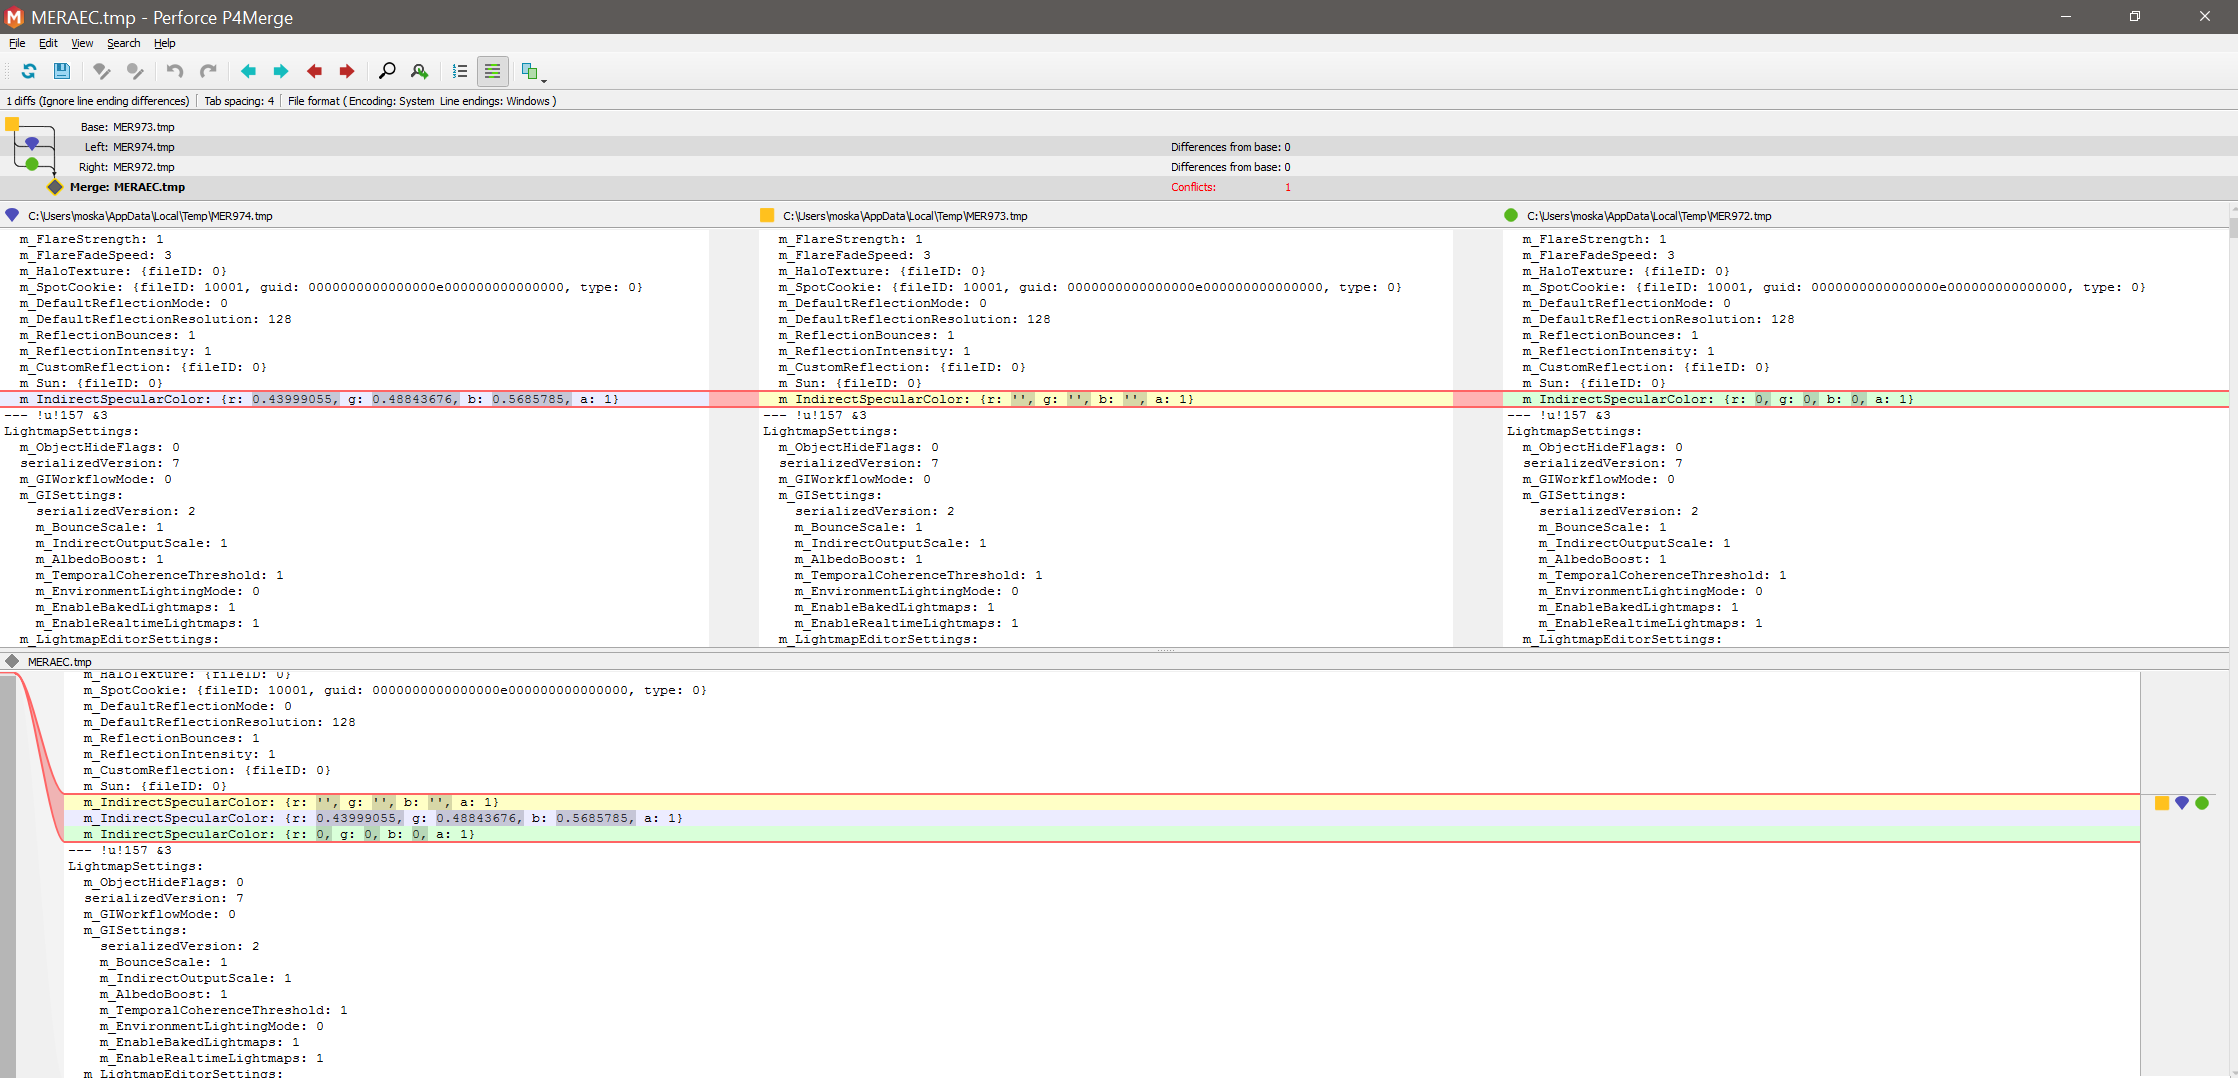
\includegraphics[width=\textwidth]{p4merge.png}
\caption{Ręczne rozwiązywanie konfliktów w projekcie gry}
\end{figure}